\section{Results and Discussion}
\label{sec:simulation_result}

\begin{table*}[t]
\centering
\caption{Selected runs for the six quadratic instances. $T$: ADMM iterations; $C$: total exact agent queries; $e_F$: relative discrepancy in the original objective at the terminal primal variables. The exact-update query count is $C_0=10T_0$. All displayed GP runs satisfy the residual tests, $T\leq2T_0$, and $e_F\leq0.01\%$. Dashes indicate that cluster-wise MTGP was not evaluated for $K=1$.}
\label{tab:main_results}
\footnotesize
\setlength{\tabcolsep}{5.1pt}
\renewcommand{\arraystretch}{1.12}
\begin{tabular}{l r rrr rrr rrr}
\toprule
& ADMM & \multicolumn{3}{c}{SOGP} & \multicolumn{3}{c}{Global MTGP} & \multicolumn{3}{c}{Cluster-wise MTGP}\\
\cmidrule(lr){2-2}\cmidrule(lr){3-5}\cmidrule(lr){6-8}\cmidrule(lr){9-11}
Instance & $T_0$ & $T$ & $C$ & $e_F$ (\%) & $T$ & $C$ & $e_F$ (\%) & $T$ & $C$ & $e_F$ (\%)\\
\midrule
Homogeneous & 26 & 52 & 186 & 0.00036 & 31 & 59 & 0.00760 & -- & -- & -- \\
Heterogeneous & 39 & 75 & 152 & 0.00624 & 50 & 75 & 0.00648 & -- & -- & -- \\
Separated, $K=2$ & 35 & 68 & 215 & 0.00123 & 36 & 74 & 0.00890 & 37 & 70 & 0.00769 \\
Separated, $K=3$ & 32 & 64 & 193 & 0.00231 & 39 & 71 & 0.00990 & 40 & 75 & 0.00792 \\
Overlapping, $K=2$ & 32 & 62 & 210 & 0.00122 & 38 & 76 & 0.00866 & 42 & 70 & 0.00979 \\
Overlapping, $K=3$ & 30 & 59 & 183 & 0.00536 & 32 & 70 & 0.00676 & 31 & 69 & 0.00518 \\
\bottomrule
\end{tabular}
\end{table*}


\subsection{Communication and Iteration Tradeoff}
Table~\ref{tab:main_results} answers \textbf{RQ1}: the selected global MTGP runs require 59--76 exact queries, reducing the baseline count by $76.25$--$80.77\%$, compared with $28.46$--$61.03\%$ for SOGP. Relative to SOGP, global MTGP uses $50.7$--$68.3\%$ fewer queries. All reported runs satisfy the residual stopping tests and the stated objective-discrepancy bound. Global MTGP takes $1.03$--$1.28$ times the exact-update iteration count, whereas SOGP takes $1.92$--$2.00$ times that count. Thus the gain is fewer exact exchanges with a modest iteration increase; it is not faster convergence than exact-update ADMM.

The effect also appears beyond a single selected setting. Across the 220 settings per instance, all global and cluster-wise MTGP runs meet the residual stopping tests within the iteration cap. The fraction satisfying all selection constraints ranges from $62.3$--$95.5\%$ for global MTGP and $65.9$--$76.8\%$ for cluster-wise MTGP, compared with $13.2$--$44.5\%$ for SOGP. These grid counts describe tuning sensitivity on the fixed instances; they are not repeated-trial success probabilities.

\begin{figure}[t]
 \centering
 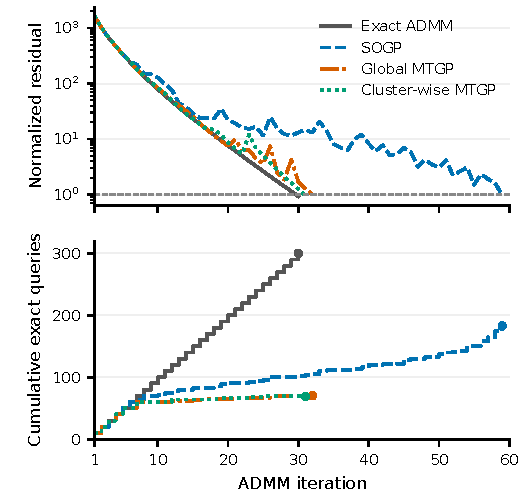
\includegraphics[width=\columnwidth]{figures/verified_diagnostic.pdf}
 \caption{Three overlapping groups, using the settings in Table~\ref{tab:main_results}. Top: maximum of the primal and dual residuals normalized by their respective stopping tolerances; the dashed horizontal line is the stopping boundary. Bottom: cumulative exact agent queries, including the 50 initialization queries. Curves end at each method's termination.}
 \label{fig:verified_diagnostic}
\end{figure}

Figure~\ref{fig:verified_diagnostic} illustrates the tradeoff on the three-group overlapping instance. Global and cluster-wise MTGP terminate after 32 and 31 iterations with 70 and 69 queries, respectively, compared with 30 iterations and 300 queries for exact-update ADMM. SOGP uses 59 iterations and 183 queries. The residual curves report algorithmic progress, while the cumulative counts separately expose the communication cost.

\subsection{Value of Known Group Labels}
For \textbf{RQ2}, the selected cluster-wise and global MTGP runs have similar communication costs. Cluster-wise MTGP saves four, six, and one additional queries for separated $K=2$, overlapping $K=2$, and overlapping $K=3$, respectively; for separated $K=3$, it uses four more queries. Its iteration count is higher in three of the four comparisons. These results do not establish a consistent communication advantage from known labels, nor do they demonstrate that overlap causes negative transfer in global MTGP. The observed gains support joint surrogate modeling across these instances, but do not by themselves verify recovery of the generating groups.

Known labels can reduce the size of each GP system. For dense exact GP factorization, let $m_k=(p+1)\sum_{i\in\mathcal C_k}n_i$ be the number of scalar observations in group $k$, and $m=\sum_km_k$. The global cost is $\mathcal O(m^3)$, whereas the total cluster-wise cost is $\mathcal O(\sum_km_k^3)$. At a fixed, balanced observation count, this gives a factor $K^2$ reduction in the leading factorization work. Actual runtime also depends on query counts, refitting, and implementation, so this is a complexity comparison rather than a measured speedup.

\subsection{Scope of the Evidence}
The study uses six synthetic quadratic instances and one optimization seed. Tuning and evaluation use the same instances, and the methods have different GP parameterizations and fitting budgets. Consequently, the results establish an empirical communication--accuracy tradeoff for these configurations, rather than convergence guarantees, generalization to unseen instances, or a causal attribution to task sharing alone. Repeated instances, a common-configuration or held-out tuning comparison, and matched-budget ablations would strengthen those broader claims.
